\chapter{Error computation\label{chap:error}}
\vspace*{-1cm}
\lettrine[lines=2, loversize=-0.1, lraise=0.1]{D}{iva} 

\minitoc


\section{Introduction}

% \section{Error field with advection}

% provided by diva, but interpretation different as the normal case
% need to add more details on this
The analysis performed with the optimised parameters should have the lowest global error, as measured by \eqref{eq:gcvbis}. Nevertheless, the spatial distribution of the error is also of interest. The latter is very easy to calculate with OI: according to \eqref{eq:erroroi} we need to apply the analysis (operator $\matr{H}$) on a vector containing the covariances of the data locations with the location where the error has to be calculated. Hence, in principle, a new analysis has to be performed for each point in which the error is requested. On the contrary, the error calculation in \diva is not trivial since the covariance functions are never explicitly specified. The object of this section is to define methods to generate error fields associated to the analysis. 

\subsection{The poor man's estimate\label{sec:poormans}}

To circumvent the main problems (unknown covariance function and repeated analysis), \citet{BRASSEUR94} estimated the error by analysing a vector of "covariances" with constant $\sigma^2$. As all "covariances" are identical, the error can be assessed in all locations with the same analysis. The advantage is the fast calculation, but the drawback is a systematic underestimation of the actual errors, since the error reduction by the overestimated covariances \eqref{eq:erroroi} is also overestimated. The poor man's error field is a very efficient way to assess data-coverage and determine the regions where the analysis cannot be trusted.

\subsection{The hybrid approach}

In this approach, the covariance vector to be analysed is calculated using the covariance function of an infinite domain \citep{BRANKART98,RIXEN00}. In an infinite domain, the error calculation is then "exact", while for more complicated domains, it is nearly exact far away from boundaries, provided no anisotropic constraint is activated. 

The problem of the approximate hybrid error calculation relies on the fact that instead of the actual covariance, only the kernel computed under the assumption of an infinite domain (without dynamic constrain) is analysed with \diva to produce the error field. Hence, for anisotropic cases (as found with advection constraints, variable length scale or near boundaries), the hybrid error field can be incoherent. This is what motivated the evaluation of the real covariance function in \diva.

\subsection{The real covariance method}

If we look back at the OI interpretation, we can place a data of value $1$ at location $\vect{r}$ and compute the analysis $\varphi_1(\vect{r}^\prime)$ at a location $\vect{r}^\prime$:
\begin{equation}
\varphi_1(\vect{r}^\prime) = {\snr \hat{B} (\vect{r},\vect{r}^\prime)\over  \snr \hat{B}(\vect{r},\vect{r}) + \hat{R}(\vect{r}) },
\end{equation}
where $\hat{B}(\vect{r},\vect{r}^\prime)$ is the non-dimensional covariance function between points $\vect{r}$ and $\vect{r}^\prime$, whereas $\hat{R}$ is the normalized observational error variance. Normalization was done respectively by the background variance $\sigma^2$ and noise $\noise^2$, yielding the signal-to-noise ratio $\snr$ previously defined. 
At the data location itself, we get the analysis
\begin{equation}
\varphi_1(\vect{r}) = {\snr \hat{B} (\vect{r},\vect{r}) \over \snr \hat{B}(\vect{r},\vect{r}) + \hat{R}(\vect{r}) }.
\end{equation}

In terms of interpretation of the covariance function as the kernel of the norm (the second term of \eqref{eq:variab}), it is the background covariance that is modified by the anisotropy and not the noise level. Hence, if we put the unit data value with a unit signal-to-noise ratio in $\vect{r}$, we directly have

\begin{equation}
\varphi_1(\vect{r}^\prime) = { \hat{B} (\vect{r},\vect{r}^\prime)\over   \hat{B}(\vect{r},\vect{r}) + 1 } \qquad \textrm{and} \qquad 
\varphi_1(\vect{r}) = { \hat{B} (\vect{r},\vect{r}) \over  \hat{B}(\vect{r},\vect{r}) + 1 }.
\end{equation}
The left-hand sides are provided by the \diva application to the unit data point in location $\vect{r}$ with unit signal-to-noise ratio and analysed in any desired location $\vect{r}^\prime$ and $\vect{r}$. From these two values, it is therefore easy to calculate the covariance function $\hat{B}$ inherently used in \diva.

For the error calculation at a point $\vect{r}$, we have the following procedure: 

\begin{enumerate}

\item Put a unit value at $\vect{r}$ and perform an analysis with $\snr=1$.

\item Save the result at the locations of the original data and of the error-calculation, where the analysis value is
\begin{equation}
\varphi_0 ~=~{ \hat{B} (\vect{r},\vect{r}) \over \hat{B}(\vect{r},\vect{r}) + 1 },
\end{equation}

\item Calculate the background variance $\hat{B}(\vect{r},\vect{r})$ at the error-field location:
\begin{equation}
\hat{B} (\vect{r},\vect{r}) = { \varphi_0 \over 1 - \varphi_0}.
\label{eq:brr}
\end{equation}

\item Calculate the covariance $\hat{B} (\vect{r},\vect{r}_i)$ between the error location and data locations. Since at the data points $i$ located at $\vect{r}_i$, \diva application provides
\begin{equation}
\varphi_i ~=~ { \hat{B} (\vect{r},\vect{r}_i) \over \hat{B}(\vect{r},\vect{r}) + 1 },
\end{equation}
the covariance $\hat{B} (\vect{r},\vect{r}_i)$ is obtained as
\begin{equation}
\hat{B} (\vect{r},\vect{r}_i)~=~{\varphi_i \over ( 1-\varphi_0 )}.
\label{eq:btildco}
\end{equation}

\end{enumerate}

Up to the multiplication constant $1/(1-\varphi_0)$, the non-dimensional covariance of a point in position $\vect{r}$ with a list of other points can therefore be obtained by putting a unit data value in $\vect{r}$ and taking the value of the analysis at the coordinates of the list of points. 


To illustrate the procedure, we take a simple case with one point in the center of the domain, and another point near the boundary.
Near the boundary, data points influence more easily the analysis because rigidity is reduced (Fig.~\ref{fig:fig4_kernel_bceffect}). This translates into a larger background variance. Error fields will therefore be larger near boundaries when there are no nearby data.
 
\begin{figure}[htpb]
\centering
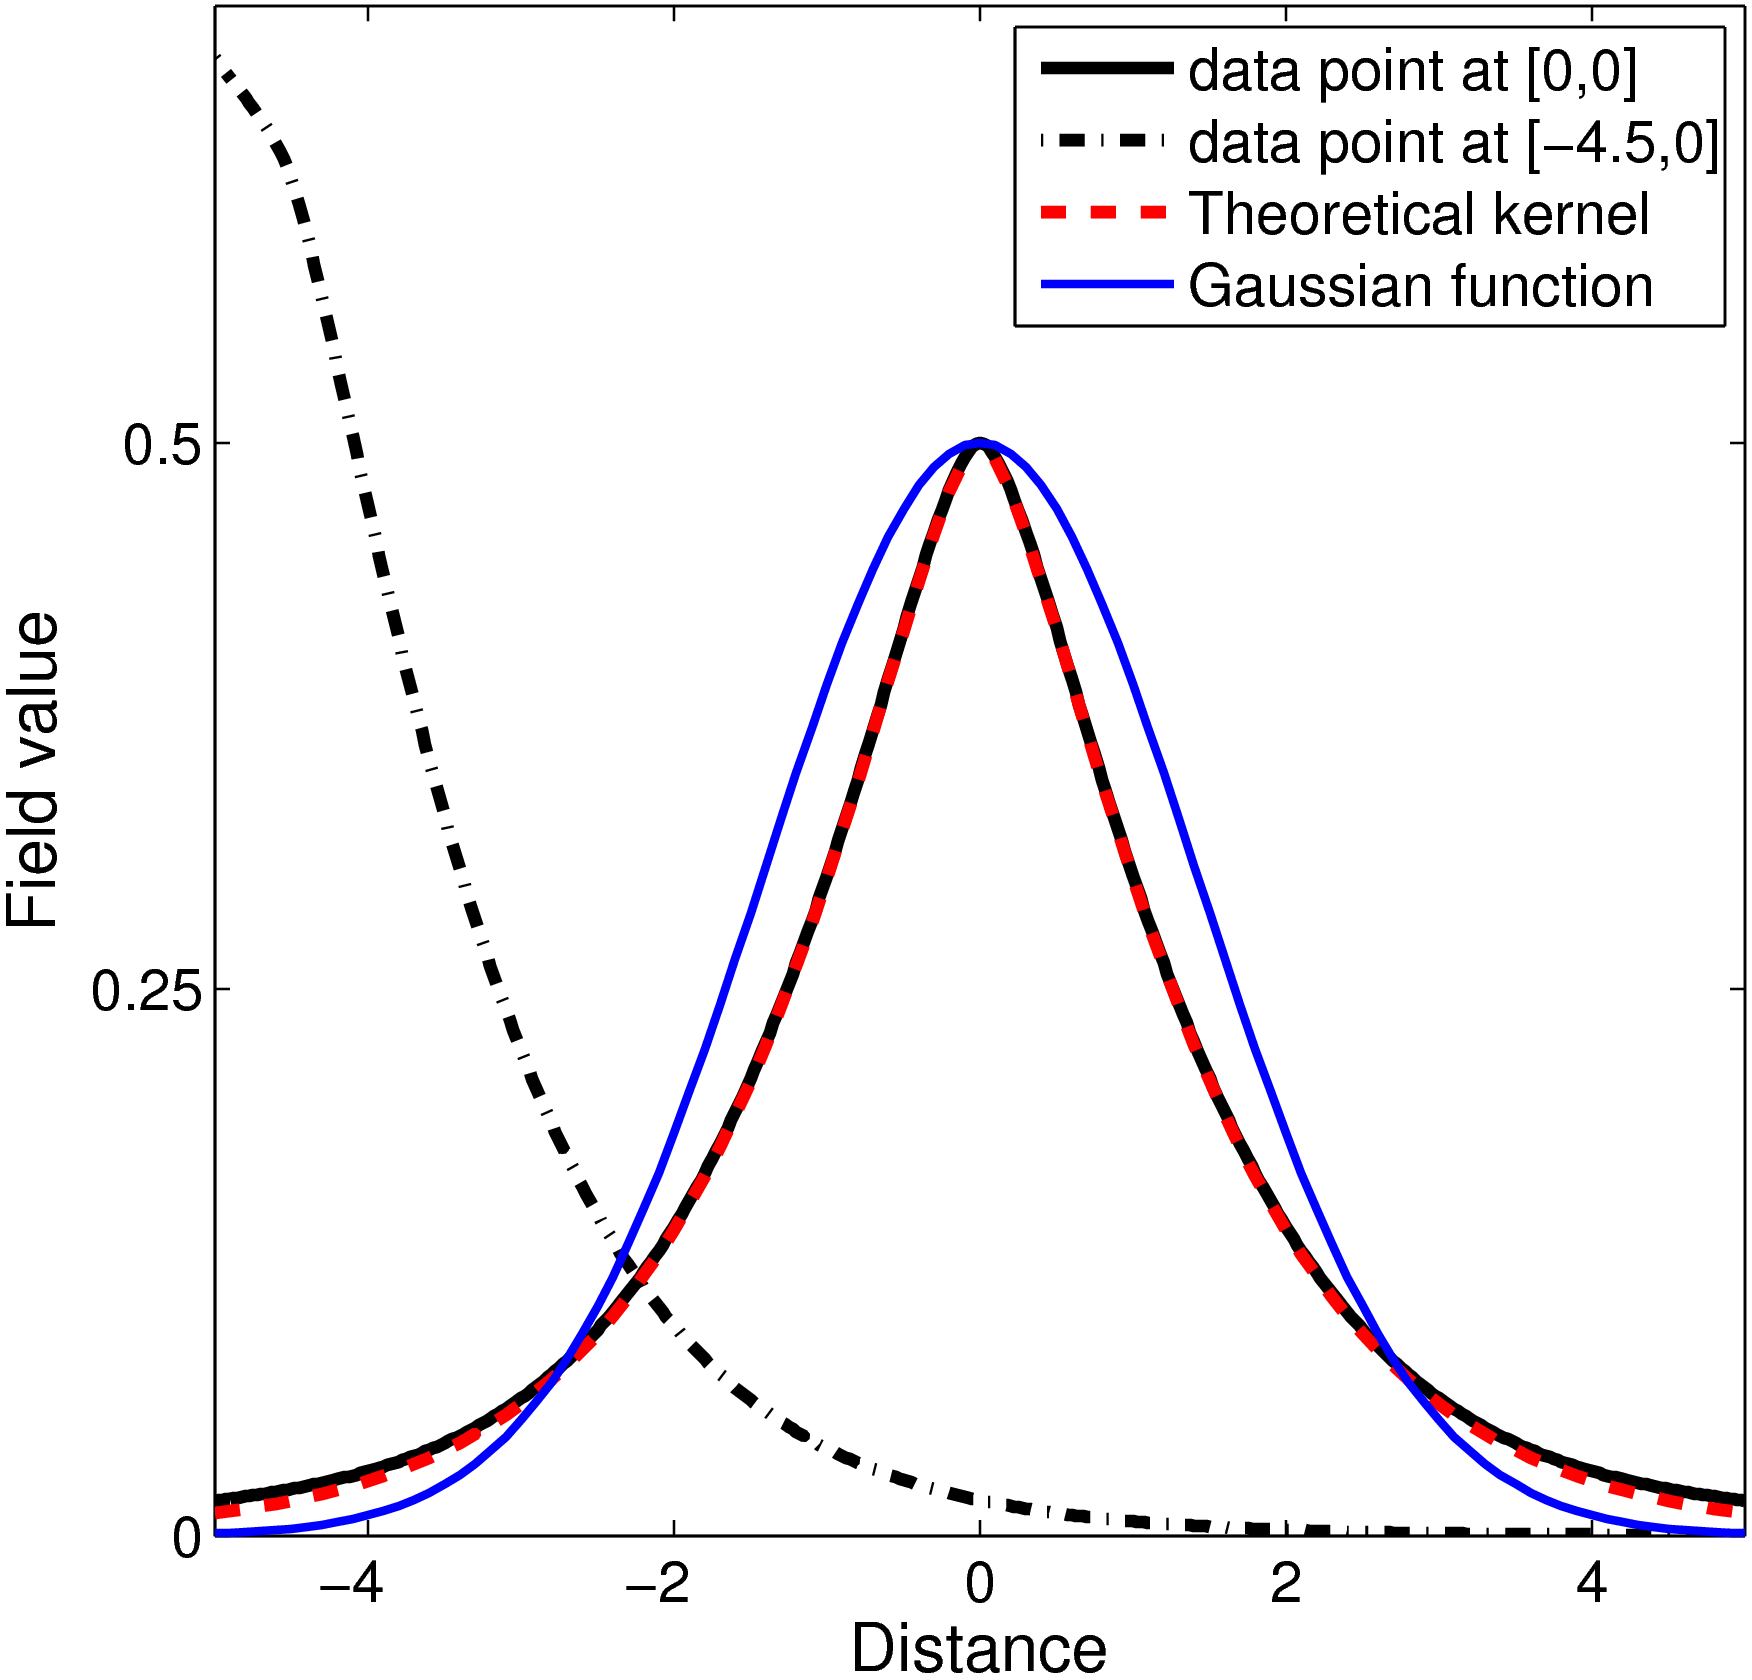
\includegraphics[width=.7\textwidth,bb=66 206 510 630]{fig4_kernel_bceffect}
\caption{Analysis in a square domain $[-5,5]\times[-5,5]$ with a point at the centre and another at $(-4.5,0)$. The signal-to-noise ratio $\snr=1$ for both cases. Note the larger analysis value near the boundary, indicating a larger background variance.
\label{fig:fig4_kernel_bceffect}}
\end{figure} 
 
 
From there, applying the correction $1/(1-\varphi_0)$, we can use the covariances as input vector for a second \diva execution, so as to perform an analysis of the covariance and getting access to the error of the analysis at the desired location. Indeed, using the equivalence of \diva and OI, if the analysis step applied to a data vector $\vect{d}$ is formally written 
\begin{equation}
\varphi_a = \matr{H} \vect{d},
\end{equation}
then the error is 
\begin{equation}
\epsilon_a^2 (\vect{r}) = \sigma^2 \hat{B}(\vect{r},\vect{r}) - \sigma^2 \matr{H} \hat{\vect{b}},
\end{equation}
where $\hat{B}(\vect{r},\vect{r})$ is the local relative background variance (calculated by \eqref{eq:brr}) and $\hat{\vect{b}}$ is a vector filled according to \eqref{eq:btildco}.

\clearpage

%------------------------------------
\section{Integrals over (sub-)domains}
%------------------------------------

Very often, we are not only interested in the analysed field itself but also in its integral over the
total domain or a sub-domain. If we have the analysis on a sufficiently fine output grid, the integral
itself is then just a sum of the values at the grid points covering the integration domain, multiplied by the
grid-cell surface. Hence we do not consider here the additional approximation brought by replacing a continuous integral by
a discrete sum. Indeed, generally the output grid is fine compared to the scales of interest
and the sum can be considered an "exact" integral. Hence, we will focus here on the error on a discrete sum of the analysed field.

\subsection{Theory}
%------------------

Formally, if $\mathbf{x}^a$ is a column vector containing the analysed field values at the grid
points defining the integration domain, the weighted sum $I$ over this values is
\begin{equation}
I~=~(\mathbf{x}^a)^T \mathbf{h}
\end{equation}
where $^{T}$ stands for the transposed vector or matrix and $\mathbf{h}$ is a column vector of the same size as
$\mathbf{x}^a$ but whose components are the weight associated with each integration point. The weight is typically the surface associated with
the integration point. For an integration over a uniform grid, the weights can without loss of generality be unit (the surface dimension can be retrieved at the end by global multiplication). 

Note that the weights here have nothing to do with the weight on data points for an analysis.

Now the analysis is not exact but has an associated random error $\mathbf{\epsilon}^a$ with respect to the true
field values $\mathbf{x}^t$:

\begin{equation}
{\mathbf{x}^a} = \mathbf{x}^t + \mathbf{\epsilon}^a
\end{equation}
On statistical average (noted $< \quad >$), we suppose the analysis is unbiased and
\begin{equation}
<{\mathbf{x}^a}> = \mathbf{x}^t 
\end{equation}
In order to calculate the error variance on the sum, we calculate the expected square distance with respect to the true sum:
\begin{equation}
\Delta^2 = < \mathbf{h}^T( {\mathbf{x}^a} - \mathbf{x}^t) ({\mathbf{x}^a} - \mathbf{x}^t )^T \mathbf{h} > = \mathbf{h}^T \, \mathbf{P}^a \, \mathbf{h}
\label{eq:errorintegral}
\end{equation}
where $\mathbf{P}^a = <\mathbf{\epsilon}^a {\mathbf{\epsilon}^a}^T >$ is the error-covariance matrix of the analysis.
We see that the spatial covariances of the analysis-error field are required to calculate the error variance on $I$. Since this
covariance matrix is not diagonal, it is not sufficient to sum up the local error values of the error fields of $\mathbf{x}^a$. The latter sum would limit
the double sum of \eqref{eq:errorintegral} to the diagonal terms of $\mathbf{P}^a$.


\subsection{Implementation}
Exploiting the equivalence of \diva and OI, we know that

\begin{equation}
\mathbf{P}^a ~=~ \mathbf{P} -  \mathbf{C}^T \left( \mathbf{B}+\mathbf{R} \right)^{-1} \mathbf{C}
\label{eq:covariance}
\end{equation}
where $\mathbf{P}$ is the covariance matrix (size $N_g\times N_g$) of the background field between the $N_g$ grid points under consideration, $\mathbf{B}$ 
the covariance matrix (size $N_d \times N_d$) of the background field between the $N_d$ data points, $\mathbf{C}$  is the
 covariance matrix (size $N_d \times N_g$) of the background field between the  data points and grid points and finally $\mathbf{R}$ is the error covariance matrix (size $N_d \times N_d$) on the data.
 
We could calculate the covariances matrices involved exactly (as done for the exact error calculation) and then calculate \eqref{eq:errorintegral} but this would be prohibitively expensive if done in a brute force approach. However when done in a clever way it is feasible.

\subsubsection{Direct approach}

Using \eqref{eq:covariance} and \label{eq:errorintegral} we can write

 \begin{equation}
 \Delta^2 = \mathbf{h}^T \, \mathbf{P} \, \mathbf{h} - \mathbf{h}^T \underbrace{\mathbf{C}^T \left( \mathbf{B}+\mathbf{R} \right)^{-1}} \, \underbrace{\mathbf{C}  \, \mathbf{h}}
 \label{eq:totalerror}
 \end{equation}
 
The term $\mathbf{C}  \, \mathbf{h}$ is readily interpreted as a columns vector containing $N_d$ elements. Element $j$ is the (weighted) sum of the covariances of all integration points with the data point $j$. The middle term is the analysis operator that provides the analysis on the grid points when providing on input a columns vector of size $N_d$. Hence the recipe to calculate $\Delta^2$ without explicitly forming the error-covariance matrices is the following:
\begin{itemize}
\item Perform a double sum on all covariances between grid points to calculate $\mathbf{h}^T \, \mathbf{P} \, \mathbf{h}$.
\item For the term to subtract, evaluate it starting from the right: form a pseudo-data vector by summing covariances of all grid points with each data point, analyse it and finally sum up the analysis at the grid points.
\end{itemize}

All we have to to is to be calculate covariance functions. This can be done with the module {\tt covar} of \diva, which allows one to calculate
a series of covariances with a single matrix inversion. Hence the recipe of calculating \eqref{eq:totalerror} includes a \diva run to calculate covariances (cost roughly equal to an analysis with full error field), followed by a second \diva run to analyse the "data" $\mathbf{C}  \, \mathbf{h}$.



\subsubsection{Hybrid approach}

A simplified versions can be used, using to some extend the fact the covariance functions in an infinite domain are known analytically when no
advection constraint or variable correlation length is activated. We can indeed introduce an approximation that makes the calculation manageable without calculating the covariances with \diva itself. Instead of using the exact covariances on the background field, we use the covariances we would find in an infinite domain with constant correlation length and without advection constraint. In this case, we know
that the correlation function $c$ between two points is
\begin{equation}
c(r) ~=~{r \over L} K_1 \left(r \over L\right)
\end{equation}
where $r$ is the distance between the two points, $L$ the correlation length and $K_1$ a Bessel function\index{Bessel function}. To get the covariance function we simply have to multiply by the variance $\sigma^2$ of the background field.

Hence we can estimate $\Delta^2$ by calculating these covariance functions between grid and data points and performing one analysis with \diva.

\subsubsection{Inflation approach}

A second simplified approach makes even stronger assumptions but shows how we can try to "extrapolate" the error estimated from the sum of the diagonal terms of $\mathbf{P}^a$ to the estimation of the double sum. To do so, we assume that the analysis error has a spatial correlation scale similar to the analysis.
This is probably too severe and we will therefore overestimate the integral error. 
Here we use a continuous formulation to calculate an approximation of $\Delta$ noted $\tilde{\Delta}$ by starting from the sum expressed as continuous integral
\begin{equation}
{\Delta}^2= {1 \over \Delta x^2 \Delta y^2} \int_D \int_D <{\epsilon}^a(x) {\epsilon}^a(x^\prime)> d x^\prime d x 
\end{equation}
where $x$ and $x^\prime$ stand for positions in the domain of integration $D$. When we suppose the covariance is isotropic and note $r$ the distance between points
$x$ and $x^\prime$ we have 
\begin{equation}
{\Delta}^2= {1 \over \Delta x^2 \Delta y^2} \int_D \int_D <{\epsilon}^a(x) {\epsilon}^a(x) > c(r) d x^\prime d x  
\end{equation}
which we can evaluate in polar coordinates the inner integral expanded to infinity to find an approximate value
\begin{equation}
\tilde{\Delta}^2= {2 \pi \over \Delta x^2 \Delta y^2} \int_D <{\epsilon}^a(x) {\epsilon}^a(x) > \int_0^{\infty}  r c(r) d r d x
\end{equation}
with the Bessel function for the correlation function $c$ this yields
\begin{equation}
\tilde{\Delta}^2= {4 \pi L^2 \over \Delta x^2 \Delta y^2} \int_D <{\epsilon}^a(x) {\epsilon}^a(x) >  d x
\end{equation}

If we had used the naive approach of neglecting the spatial covariances, the double sum would have been restricted to a simple sum on diagonal and we would calculated the underestimated error 
\begin{equation}
\tilde{\tilde{\Delta}}^2= {1 \over \Delta x \Delta y} \int_D <{\epsilon}^a(x) {\epsilon}^a(x) >  d x.
\end{equation}
Hence we see that we should apply an inflation factor of $\sqrt{{4 \pi L^2 \over \Delta x \Delta y}}$ on $\tilde{\tilde{\Delta}}$ to get a better estimate of the error standard deviation. In practice  this inflation factor is probably a little too high (we assumed the analysis error to have the same correlation length as the analysis while in reality it is generally smaller and we extended one of the integrals to an infinite domain, adding up more errors).


\subsection{Use}

All approaches were implemented into \command{divaintegral}. If there is a file\\ 
\file{./input/integrationpoints.dat}, it will be used.
Otherwise it will be created (and put in the \directory{./output}), based on the analysis on the output grid. This files must contain $x,y,val,1,h$. If the file did not exist but was created, it will pass through an execution of \command{divaintegral}. 
\command{divaintegral} can be edited by the user to chose special points for the integration (for example only those points for which the analysis is positive, or points that fall in a given square etc). 

When {\textit ispec } is negative, the full covariance calculation will be used. When {\textit ispec } is positive, the hybrid covariance calculation will be used.

When called with the optional argument \texttt{-naive}, it also calculates the simple sum of the diagonal term of the analysis error variance. The error field itself is calculated with the methods specified by \texttt{ispec}. 

\begin{lstlisting}[style=Bash]
[charles@gher13 divastripped]$ divaintegral -naive
\end{lstlisting}

The output files generated are:
\begin{itemize}
\item \file{./output/integral.dat} contains the integral value, the surface of the integration domain and the average value (integral divided by surface).
\item \file{./output/erroronintegral.dat} contains the error standard deviation on the integral, in the same units as the integral.
\item \file{./output/erroronintegralnaive.dat} contains the naive approach summing only the diagonal terms, the inflation factor and the inflated error. Units are the same as the integral.
\end{itemize}

Units are units of the variable multiplied by the units of $x$ and $y$ of the data and contour file, when no coordinate change is performed or the option {\tt icoordchange = -xscale} was used.

When {\tt icoordchange} is one or two, the surface units of the output are m$^2$.

Note that the tool is not designed for use with the poor man's error calculation (\texttt{ispec}>10, Section~\ref{sec:poormans}).

\subsection{Interna}
%-------------------

\begin{itemize}

\item \texttt{gridpointlist.a} creates a list of wet points of the analysis grid. 

Input: \texttt{fort.20} gridded gher file, \texttt{fort.21} corresponding to \file{GridInfo.dat}.\\ 
Output: \texttt{fort.22} list of points with value of analysis on wet points only (x,y,val,1,1).

\item \texttt{erroronintegrals.a} calculates the double sum on background covariance and prepares the pseudo-data (sum of covariances of all grid points with a  data point).

Input: \texttt{fort.10} list of grid points for the integral (including third column for value of field), \texttt{fort.11} data file, \texttt{fort.5} scale lc datacol.\\
Output: \texttt{fort.14} double sum, \texttt{fort.12} pseudo-data vector.
\end{itemize}

For exact covariance functions, 

\begin{lstlisting}[style=Bash]
[charles@gher13 divastripped]$ divacalc -pfsum
\end{lstlisting}

is executed, which allows the use the full suite of \diva parameters (including for example advection constraint). Internally, as we need the covariance of all integral points with all integral points and data locations, we provide to {\tt divacalc -pfsum} in input "data" which are the integration points and ask in addition values in a list of points (which are the original data location).

